%(BEGIN_QUESTION)
% Copyright 2007, Tony R. Kuphaldt, released under the Creative Commons Attribution License (v 1.0)
% This means you may do almost anything with this work of mine, so long as you give me proper credit

Her vises responsen til en prosess på en serie trinnendringer i regulatorutgangen (alle gjort mens regulatoren stod i ``manuell'' modus). Hva kan du, basert på observasjonene dine, fastslå om prosessen og tilhørende instrumentering?

$$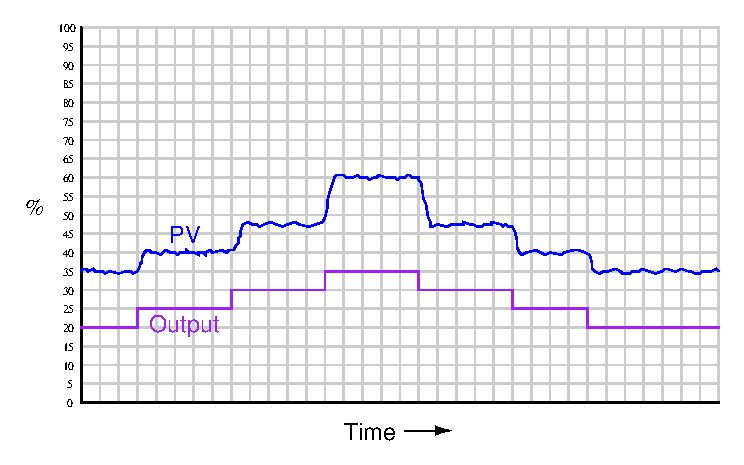
\includegraphics[width=15.5cm]{i01651x01.eps}$$

Er denne prosessresponsen et potensielt problem? Hvis ja, hvilken type problem er det?

\underbar{file i01651}
%(END_QUESTION)





%(BEGIN_ANSWER)

Prosessen (som helhet) har variabel forsterkning. Hvis prosessen har variabel forsterkning, betyr det at total sløyfeforsterkning vil øke og minke avhengig av PV-verdien. Det betyr at sløyfen vil være mindre stabil ved noen PV-verdier enn ved andre.

Dette kan skyldes sterk ikke-linearitet i transmitteren eller i en signalomformer, en reguleringsventil med ikke-lineær installert karakteristikk (i dette tilfellet en equal-percent {\it installert} karakteristikk -- lite sannsynlig), eller noe som er iboende i selve prosessen (mest sannsynlig).

For å motvirke denne forsterkningsustabiliteten må regulatoren (eller et annet element i sløyfen) konfigureres med en invers forsterkningsrespons, slik at sløyfeforsterkningen holdes konstant. En regulator med {\it adaptiv forsterkning} kan brukes til dette, eller eventuelt en annen ventilkarakteristikk kan installeres.

%(END_ANSWER)





%(BEGIN_NOTES)


%INDEX% Control, PID tuning: step change (output) revealing variable gain

%(END_NOTES)
